\newpage
\section{Datenbankentwurf}
\def \currentAuthor{Elias Gabl}

\subsection{Tabellenbeschreibung OSTicket}

In dieser Dokumentation finden Sie eine grobe Beschreibung der Datenbank des Systems OS Ticket. OS Ticket ist ein Ticketsingsystem das für einfache Support Anwendung Entwickelt worden ist. Die Datenbank besteht aus 59 Tabellen von diesen sind manche nicht mehr aktuell bzw. werden nicht mehr gebraucht aber sind dennoch vorhanden. Daher werden in dieser Dokumentation nur die wichtigsten Tabellen der Datenbank beschrieben.\\
Bei gewissen Spalten ist es leider nicht möglich den Inhalt anzugeben da es keine gute Dokumentation der Datenbank gibt und man den Inhalt der Spalten aus dem Kontext schließen muss.
\newline
\newline
An dieser Stelle sollte eigentlich ein Datenmodell sein aber da dieses von OSTicket recht groß und komplex ist hat es hier nicht Platz aber Sie finden es auf dem mitgelieferten Datenträger.(Der Dateiname ist: OSTicketDB.mwb).

\subsubsection{ost\_config}

In dieser Tabelle werden wichtige Informationen über das System OSTicket gespeichert. Die Werte werden mit einem Schlüssel in die Datenbank gespeichert (Key und Value).
Diese Tabelle hat keine Referenz zu anderen Tabellen.

\begin{table}[h]
	\begin{tabular}{|p{3.5cm}|p{4cm}|p{6.2cm}|}
		\hline
		\textbf{Column Name:} & \textbf{Datatype:} & \textbf{Content:}\\
		\hline
		id & INT(11) & Eindeutige ID der Information. Dieser Wert ist rein technisch und hat  neben der Eindeutigkeit keine weitere 
		Aussagekraft. \\
		\hline
		namespace & VARCHAR(64) & \\
		\hline
		key & VARCHAR(64) & Key der Information um die Suche zu erleichtern\\
		\hline
		value & TEXT & Informations Inhalt\\
		\hline
		updated & DATETIME & Erstelldatum der Information\\
		\hline
	\end{tabular}
	\caption{tab:ost-config}
\end{table}
\label{tab:ost_config}
\newpage


\subsubsection{ost\_attachment}

Sämtliche Informationen über den Anhang eines Tickets finden sich in dieser Tabelle. Dies beinhaltet den Datentyp, Name, und id des Anhanges. 

\begin{table}[h]
	\begin{tabular}{|p{3.5cm}|p{4cm}|p{6.2cm}|}
		\hline
		\textbf{Column Name:} & \textbf{Datatype:} & \textbf{Content:} \\
		\hline
		id & INT(10) & Eindeutige ID des Anhanges. Dieser Wert ist rein technisch und hat  neben der Eindeutigkeit keine weitere  \\
		\hline
		object\_id & int(11) & Referenz auf ein Object das dem Anhang übergeben wird \\
		\hline
		type & CHAR(1) & Datentyp des Anhanges hat \\
		\hline
		file\_id & int(11) & Referenz auf das File das sich im Anhang befindet\\
		\hline
		name & VARCHAR(255) & Name des Anhanges \\
		\hline
		inline & TINYINT(1) & Beschreibt den Zitierstil des Anhangs \\
		\hline
		lang & VARCHAR(16) & Die Sprache in der Abteilung \\
		\hline
	\end{tabular}
	\caption{tab:ost-attachment}
\end{table}
\label{tab:ost_attachment}

\newpage

\subsubsection{ost\_canned\_response}

In dieser Tabelle werden vorgefertigte Antworten für Tickets gespeichert. Über die Antwort wird der Titel, die Sprache, der Inhalt, Erstelldatum und das Änderungsdatum gespeichert.

\begin{table}[h]
	\begin{tabular}{|p{3.5cm}|p{4cm}|p{6.2cm}|}
		\hline
		\textbf{Column Name:} & \textbf{Datatype:} & \textbf{Content:}\\
		\hline
		canned\_id & INT(10) & Eindeutige ID der Nachricht. Dieser Wert ist rein technisch und hat  neben der Eindeutigkeit keine weitere 
		Aussagekraft.\\
		\hline
		dept\_id & int(10) & Referenz auf die Abteilung die diese Nachricht verwenden können\\
		\hline
		isenabled & TINYINT(1) & Ob die Nachricht freigegeben ist oder nicht.\\
		\hline
		titel & VARCHAR(255) & Titel der Nachricht\\
		\hline
		response & TEXT & Text den die Nachricht beinhaltet\\
		\hline
		lang & VARCHAR(16) & Sprache der Nachricht\\
		\hline
		notes & TEXT & Anmerkung zur Nachricht\\
		\hline
		created & DATETIME & Erstelldatum der Nachricht\\
		\hline
		updated & DATETIME & Änderungsdatum der Nachricht\\
		\hline
	\end{tabular}
	\caption{tab:ost-canned-response}
\end{table}
\label{tab:ost_canned_response}

\newpage

\subsubsection{ost\_content}

In dieser Tabelle werden Inhalte der Seiten gehalten. Es wird angeben ob der Inhalt aktiv ist oder nicht. Jeder Inhalt hat auch eine Titel und eine Body. Es werden auch noch der Typ und das Erstell/Änderungsdatum angegeben.

\begin{table}[h]
	\begin{tabular}{|p{3.5cm}|p{4cm}|p{6.2cm}|}
		\hline
		\textbf{Column Name:} & \textbf{Datatype:} & \textbf{Content:}\\
		\hline
		id & INT(10) & Eindeutige ID des Contents. Dieser Wert ist rein technisch und hat  neben der Eindeutigkeit keine weitere 
		Aussagekraft.\\
		\hline
		isactive & TINYINT(1) & Gib an ob der Inhalt aktiv ist oder nicht\\
		\hline
		type & VARCHAR(32) & Gib den Typ vom Inhalt an\\
		\hline
		name & VARCHAR(255) & Name vom Inhalt\\
		\hline
		body & TEXT & Der Bodyinhalt des Seiten Content\\
		\hline
		notes & TEXT & Anmerkungen zum Content\\
		\hline
		created & DATETIME & Erstelldatum des Content\\
		\hline
		updated & DATETIME & Änderungsdatum des Content\\
		\hline
	\end{tabular}
	\caption{tab:ost-content}
\end{table}
\label{tab:ost_content}

\newpage

\subsubsection{ost\_department}

Diese Tabelle speichert Informationen über eine Abteilung. Jede Abteilung hat einen Namen und eine Signatur. Ein Feld das angibt ob die Abteilung öffentlich ist oder nicht. Es wird auch festgehalten zu welcher Gruppe die Abteilung gehört und wann die Abteilung erstellt worden ist.

\begin{table}[h]
	\begin{tabular}{|p{3.5cm}|p{4cm}|p{6.2cm}|}
		\hline
		\textbf{Column Name:} & \textbf{Datatype:} & \textbf{Content:}\\
		\hline
		id & INT(10) & Eindeutige ID der Abteilung. Dieser Wert ist rein technisch und hat  neben der Eindeutigkeit keine weitere 
		Aussagekraft.\\
		\hline
		pid & INT & Referenz zu der Tabelle ost\_plugin \\
		\hline
		tpl\_id & INT(10) & Referenz zum verwendeten Template für die Abteilung\\
		\hline
		sla\_id & INT(10) & Referenz zur verwendeten Sla Vorlage\\
		\hline
		email\_id & INT(10) & Referenz zu der Verwendeten E-Mail der Abteilung\\
		\hline
		autores\_email\_id & INT(10) & \\
		\hline
		manager\_id & INT(10) & Referenz zum User der zum Manager der Abteilung ernannt wurde\\
		\hline
		flags & INT(10) & \\
		\hline
		name & VARCHAR(128) & Name der Abteilung \\
		\hline
		signature & TEXT & Signatur der Abteilung \\
		\hline
		ispublic & TINYINT(1) & Gib an ob die Abteilung öffentlich sichtbar ist \\
		\hline
		group\_membership & TINYINT(1) & Gib an zu welcher Gruppe die Abteilung gehört \\
		\hline
		ticket\_auto\_ response & TINYINT(1) & Das vordefinierte Standartticket der Abteilung \\
		\hline
		message\_auto\_ response & TINYINT(1) & Die vordefinierte Standartantwort der Abteilung auf Tickets \\
		\hline
		path & VARCHAR & Pfad der Abteilung\\
		\hline
		updated & INT(10) & Änderungsdatum der Abteilung\\
		\hline
		created & INT(10) & Erstelldatum der Abteilung\\
		\hline
	\end{tabular}
	\caption{tab:ost-department}
\end{table}
\label{tab:ost_department}

\newpage


\subsubsection{ost\_faq}

In dieser Tabelle werden die meist gestellten Fragen und die Antworten dazu gespeichert. Weiteres werden noch Schlüsselwörter und Anmerkungen zur Frage gespeichert.

\begin{table}[h]
	\begin{tabular}{|p{3.5cm}|p{4cm}|p{6.2cm}|}
		\hline
		\textbf{Column Name:} & \textbf{Datatype:} & \textbf{Content:}\\
		\hline
		faq\_id & INT(10) & Eindeutige ID der Frage. Dieser Wert ist rein technisch und hat  neben der Eindeutigkeit keine weitere 
		Aussagekraft.\\
		\hline
		category\_id & INT(10) & Referenz zu der Kategorie der die Frage zugeordnet ist  \\
		\hline
		ispublished & TINYINT(1) & Gib an ob die Frage öffentlich abrufbar ist oder nicht\\
		\hline
		question & VARCHAR(255) & Die Frage\\
		\hline
		answer & TEXT & Die Antwort zur Frage\\
		\hline
		keywords & TINYTEXT & Die Schlüsselwörter der Frage \\
		\hline
		notes & TEXT & Anmerkung zur Frage\\
		\hline
		created & DATETIME & Erstelldatum der Frage\\
		\hline
		updated & DATETIME & Änderungsdatum der Frage\\
		\hline
	\end{tabular}
	\caption{tab:ost-faq}
\end{table}
\label{tab:ost_faq}

\newpage

\subsubsection{ost\_staff}

Diese Tabelle hält sämtliche Informationen über die Staff Mitglieder des Systems OSTicket. Es wird der Vorname, Nachname, Username, das Passwort, die Email-Adresse, die Telefonnummer, die Sprache, ob das Mitglied aktiv ist, ob das Mitglied ein Administrator ist usw. gespeichert.
Die Tabelle enthält auch Informationen über die Abteilung und die Rolle des Mitglieds.


\begin{table}[h]
	\begin{tabular}{|p{3.5cm}|p{4cm}|p{6.2cm}|}
		\hline
		\textbf{Column Name:} & \textbf{Datatype:} & \textbf{Content:}\\
		\hline
		staff\_id & INT(11) & Eindeutige ID des Mitgliedes. Dieser Wert ist rein technisch und hat neben der Eindeutigkeit keine weitere 
		Aussagekraft.\\
		\hline
		dept\_id & INT(10) & Referenz zur Abteilung des Mitgliedes \\
		\hline
		role\_id & INT(10) & Referenz zur Rolle des Mitgliedes\\
		\hline
		username & VARCHAR(32) & Der Username des Mitgliedes\\
		\hline
		firstname & VARCHAR(32) & Der Vorname des Mitgliedes\\
		\hline
		lastname & VARCHAR(32) &  Der Nachname des Mitgliedes\\
		\hline
		passwd & VARCHAR(128) & Das Passwort des Mitgliedes in Hash Form \\
		\hline
		backend & VARCHAR(32) & \\
		\hline
		email & VARCHAR(128) & Die Email-Adresse des Mitgliedes \\
		\hline
		phone & VARCHAR(24) & Die Telefonnummer des Mitgliedes \\
		\hline
		phone\_ext & VARCHAR(6) & Referenz zur Email an die, die Info zum Ticketeingang geschickt wird \\
		\hline
		mobile & VARCHAR(24) & Die Handynummer des Mitgliedes \\
		\hline
		signature & TEXT & Die Signatur des Mitgliedes \\
		\hline
		lang & VARCHAR(16) & Die Sprache des Mitgliedes \\
		\hline
		timezone & VARCHAR(64) & Die Zeitzone in der sich das Mitglied befindet \\
		\hline
		locale & VARCHAR(16)& Wo sich das Mitglied genau befindet(Ort, Stadt, Land) \\
		\hline
		notes & TEXT & Anmerkungen zum Mitglied\\
		\hline
		isactive & TINYINT(1) & Gib an ob das Mitglied aktiv ist\\
		\hline
		isadmin & TINYINT(1) & Gib an ob das Mitglied ein Administrator ist\\
		\hline
			\end{tabular}
			\caption{tab:ost-staff}
		\end{table}
		\label{tab:ost_staff}
		\newpage
		\begin{table}[h]
			\begin{tabular}{|p{3.5cm}|p{4cm}|p{6.2cm}|}
		\hline
		isvisible & TINYINT(1) & Gib an ob das Mitglied für andere sichtbar ist \\
		\hline
		onvacation & TINYINT(1) & Gib an ob der Mitarbeiter im Urlaub ist \\
		\hline
		assigned\_only & TINYINT(1) & \\
		\hline
		show\_assigned\_ tickets & TINYINT(1) & Hat das Mitglied zugeteilte Tickets \\
		\hline
		changed\_passwd & TINYINT(1) & Gib an ob das Mitglied das Passwort schon mal geändert hat\\
		\hline
		max\_page\_size & INT(11) & Gibt die maximale Anzahl an Tickets an die auf der Übersichtsseite des Mitgliedes angezeigt werde \\
		\hline
		auto\_refresh\_rate & INT(10) & Gib die Taktrate an wie oft die Übersichtsseite des Mitgliedes automatisch aktualisiert werden soll \\
		\hline
		default\_signature\_ type & ENUM('none', 'mine', 'dept') & Gib die default Signatur bei der Beantwortung eines Tickets an \\
		\hline
		default\_paper\_size & ENUM('Letter', 'Legal', 'Ledger', 'A4', 'A3') & Gib das default Format der Antwort auf ein Ticket an \\
		\hline
		extra & TEXT & Hier können zusätzliche Informationen über das Mitglied gespeichert werden \\
		\hline
		permissions & TEXT & Die Zugriffsrechte des Mitgliedes \\
		\hline
		created & DATETIME & Erstelldatum des Mitgliedes \\
		\hline
		lastlogin & DATETIME & Datum an dem sich das Mitglied zuletzt angemeldet hat \\
		\hline
		passwdreset & DATETIME & Datum vom letzten rücksetzten des Passwortes \\
		\hline
		updated & DATETIME & Änderungsdatum des Mitgliedes \\
		\hline
	\end{tabular}
	\caption{tab:ost-staff2}
\end{table}
\label{tab:ost_staff2}

\newpage

\subsubsection{ost\_ticket}

Sämtlicher Informationen über ein Ticket. Dazu gehören der User der das Ticket abgesetzt hat, die Erkennungsnummer, die Email-Adresse des Absenders, das Thema des Tickets und wer es bearbeiten muss. Es gibt auch ein Feld das speichert ob man auf das Ticket schon geantwortet hat, wann es erstellt und gegebenenfalls verändert worden ist und ob es schon geschlossen worden ist.


\begin{table}[h]
	\begin{tabular}{|p{3.5cm}|p{4cm}|p{6.2cm}|}
		\hline
		\textbf{Column Name:} & \textbf{Datatype:} & \textbf{Content:}\\
		\hline
		ticket\_id & INT(11) & Eindeutige ID des Tickets. Dieser Wert ist rein technisch und hat  neben der Eindeutigkeit keine weitere 
		Aussagekraft.\\
		\hline
		number & VARCHAR(20) & Ticket Erkennungsnummer \\
		\hline
		user\_id & INT(11) & Referenz zum User der das Ticket abgesetzt hat.\\
		\hline
		user\_email\_id & INT(11) & Referenz zur Email-Adresse des Users der das Ticket abgesetzt hat\\
		\hline
		status\_id & INT(10) & Referenz zum Status des Tickets\\
		\hline
		dept\_id & INT(10) &  Referenz zur Abteilung der das Ticket zugewiesen wurde\\
		\hline
		sla\_id & INT(10) & Referenz zum Sla des Tickets\\
		\hline
		topic\_id & INT(10) & Referenz zum Thema dem das Ticket zugeordnet worden ist\\
		\hline
		staff\_id & INT(10) & Referenz zur Tabelle ost\_staff \\
		\hline
		team\_id & INT(10) & Referenz zum Team dem das Ticket zugewiesen worden ist \\
		\hline
		email\_id & INT(10) & Referenz zur Email an die, die Info zum Ticketeingang geschickt wird \\
		\hline
		lock\_id & INT(10) & Referenz zur Tabelle ost\_lock \\
		\hline
		flags & INT(10) &  \\
		\hline
		ip\_address & VARCHAR(64) & Die IP-Adresse von der das Ticket abgesetzt worden ist \\
		\hline
			\end{tabular}
			\caption{tab:ost-ticket}
		\end{table}
		\label{tab:ost_ticket}
		\newpage
		\begin{table}[h]
			\begin{tabular}{|p{3.5cm}|p{4cm}|p{6.2cm}|}
		\hline
		source & ENUM(Web, Email, Phone, API, Other) &\\
		\hline
		source\_extra & VARCHAR(40)&\\
		\hline
		isoverdue & TINYINT(1) & Gib an ob der Bearbeiter überfällig mit der Bearbeitung ist\\
		\hline
		isanswered & TINYINT(1) & Gib an ob dem Absender des Tickets schon geantwortet wurde\\
		\hline
		duedate & DATETIME & Gib an bis wann das Ticket bearbeitet sein sollte\\
		\hline
		est\_duedate & DATETIME & Bis wann es geplant ist das Ticket bearbeitet zu haben \\
		\hline
		reopened & DATETIME & Gib an wann ein geschlossenes Ticket zuletzt geöffnet worden ist \\
		\hline
		closed & DATETIME & Speichert das Datum an dem das Ticket geschlossen worden ist \\
		\hline
		lastupdate & DATETIME & Gib das letzte Änderungsdatum an \\
		\hline
		created & DATETIME & Erstelldatum des Tickets\\
		\hline
		updated & DATETIME & Änderungsdatum des Tickets\\
		\hline
	\end{tabular}
	\caption{tab:ost-ticket2}
\end{table}
\label{tab:ost_ticket2}

\newpage


\subsubsection{ost\_user}

Hier werden die User gespeichert die keine Mitglieder sind. Diese User können im OS Ticketsystem nur Tickets abschicken. Es wird der Name, der Status und wann er erstellt wurde gespeichert. Weiteres kann er auch einer Organisation zugeordnet werden.

\begin{table}[h]
	\begin{tabular}{|p{3.5cm}|p{4cm}|p{6.2cm}|}
		\hline
		\textbf{Column Name:} & \textbf{Datatype:} & \textbf{Content:}\\
		\hline
		id & INT(10) & Eindeutige ID des Users. Dieser Wert ist rein technisch und hat  neben der Eindeutigkeit keine weitere 
		Aussagekraft.\\
		\hline
		org\_id & INT(10) & Referenz auf die Organisation die der User zugeordnet ist\\
		\hline
		default\_email\_id& INT(10) & \\
		\hline
		status & INT(10) & Gibt den Status des Users an\\
		\hline
		name & TEXT & Name des Users\\
		\hline
		created & DATETIME & Erstelldatum des Users\\
		\hline
		updated & DATETIME & Änderungsdatum des Users\\
		\hline
		
	\end{tabular}
	\caption{tab:ost-user}
\end{table}
\label{tab:ost_user}

\newpage

\subsubsection{ost\_user\_account}

Hier wird auf Basis der ost\_user Tabelle ein Account abgespeichert.Der Account enthält eine Referenz auf einen User. Der Account besteht aus folgenden Informationen: Status des Users, die Sprache, in welcher Zeitzone er sich aufhält, den Username, das Passwort und wann er registriert wurde.

\begin{table}[h]
	\begin{tabular}{|p{3.5cm}|p{4cm}|p{6.2cm}|}
		\hline
		\textbf{Column Name:} & \textbf{Datatype:} & \textbf{Content:}\\
		\hline
		id & INT(11) & Eindeutige ID des Accounts. Dieser Wert ist rein technisch und hat  neben der Eindeutigkeit keine weitere 
		Aussagekraft.\\
		\hline
		user\_id & INT(10) & Referenz auf den User dem der Account gehört\\
		\hline
		status& INT(11) & Den Status des Users \\
		\hline
		timezone & VARCHAR(64) & Gibt die Zeitzone an in dem sich der User befindet\\
		\hline
		lang & VARCHAR(16) & Die Sprache des Users\\
		\hline
		username & VARCHAR(64) & Username des Users\\
		\hline
		passwd & VARCHAR(128) & Das Passwort des Users in Hash form\\
		\hline
		backend & VARCHAR(32) &\\
		\hline
		extra & TEXT & Zusatz Informationen zum User\\
		\hline
		registered & TIMESTAMP & Hält fest wann sich der User registriert hat\\
		\hline
		
	\end{tabular}
	\caption{tab:ost-user-account}
\end{table}
\label{tab:ost_user_account}

\newpage

\subsubsection{ost\_ticket\_priotity}

Diese Tabelle enthält alle Informationen über die Priorität die ein Ticket haben kann.
Im gesamten kann ein Ticket eine von vier Prioritäten haben.

\begin{table}[h]
	\begin{tabular}{|p{3.5cm}|p{4cm}|p{6.2cm}|}
		\hline
		\textbf{Column Name:} & \textbf{Datatype:} & \textbf{Content:}\\
		\hline
		priority\_id & TINYINT(4) & Eindeutige ID der Priorität. Dieser Wert ist rein technisch und hat  neben der Eindeutigkeit keine weitere Aussagekraft.\\
		\hline
		priority & VARCHAR(60) & Beschreibt die Priorität\\
		\hline
		priority\_desc & VARCHAR(30) & Leg fest wie die Prioritäten geordnet werden \\
		\hline
		priority\_color & VARCHAR(7) & Leg die Farbe der Prioritäten fest\\
		\hline
		priority\_urgency & TINYINT(1) & Leg fest welche Dringlichkeit die Priorität hat \\
		\hline
		ispublic & TINYINT(1) & Gib an ob die Priorität öffentlich ist oder nicht\\
		\hline
	\end{tabular}
	\caption{tab:ost-ticket-priotity}
\end{table}
\label{tab:ost_ticket_priotity}

\newpage

\subsubsection{ost\_help\_topic}

Diese Tabelle speichert die Hilfethemen. Es kann jedem Thema eine bestimmte Priorität zugeordnet werden. Weiter könne Themen auch bestimmten Abteilungen, Teams, Administratoren oder Mitarbeiter zugeteilt werden.   

\begin{table}[h]
	\begin{tabular}{|p{3.5cm}|p{4cm}|p{6.2cm}|}
		\hline
		\textbf{Column Name:} & \textbf{Datatype:} & \textbf{Content:}\\
		\hline
		topic\_id & INT(11) & Eindeutige ID des Hilfsthemas. Dieser Wert ist rein technisch und hat  neben der Eindeutigkeit keine weitere Aussagekraft.\\
		\hline
		topic\_pid & INT(10) & Referenz zu einem Plugin für das Thema\\
		\hline
		isactive & TINYINT(1) & Leg fest ob das Thema aktiv ist oder nicht \\
		\hline
		ispublic & TINYINT(1) & leg fest ob das Thema für User zur Verfügung steht\\
		\hline
		noautoresp & TINYINT(3) & \\
		\hline
		flags & INT(10) & \\
		\hline
		status\_id & INT(10) & Referenz zu dem Status \\
		\hline
		priotity\_id & TINYINT(4) & Referenz zu einem Plugin für das Thema\\
		\hline
		topic\_id & INT(10) & Referenz zu einem Plugin für das Thema\\
		\hline
		topic\_id & INT(10) & Referenz zu einem Plugin für das Thema\\
		\hline
		topic\_id & INT(10) & Referenz zu einem Plugin für das Thema\\
		\hline
		topic\_id & INT(10) & Referenz zu einem Plugin für das Thema\\
		\hline
		topic\_id & INT(10) & Referenz zu einem Plugin für das Thema\\
		\hline
		topic\_id & INT(10) & Referenz zu einem Plugin für das Thema\\
		\hline
		
	\end{tabular}
	\caption{tab:ost-help-topic}
\end{table}
\label{tab:ost_help_topic}

\newpage


\subsection{Beschreibung der Datenbankanbindung von OSTicket}
Die Datenbankanbindung in diesem System ist in der Klasse mysqli.php verankert. In dieser Klasse befinden sich Funktionen um eine Datenbankverbindung herzustellen, eine Query abzusetzen und die Verbindung wieder zu trennen.
Um diese Funktionen nutzen zu können muss die Klasse mysqli.php einfach, indem zu bearbeiteten Quellcode, mit einem Include Statement eingebunden werden.
Die Klasse besitzt im gesamten eine globale Variable namens \$\_\_db und 32 Funktionen. Die Variabel wird am Anfang der Klasse mit dem Wert Null Initialisiert und nach dem Aufrufen der db\_connect Funktion hält sie eine Mysqli Objekt.
Im folgenden Abschnitt werden die wichtigsten Funktionen im Detail beschrieben.

\subsubsection{function db\_connect}
Diese Funktion stellt die Verbindung zu einer Datenbank her. Um eine Verbindung herstellen zu können benötigt sie folgende Parameter:
	\begin{itemize}
		\item \textbf{\$host} ist die Hostadresse unter der die Datenbank erreicht werden kann.
		\item \textbf{\$user} ist ein User der die benötigen Rechte hat um lesend und schreiben auf die Datenbank zugreifen zu können.
		\item \textbf{\$passwd} ist das Passwort des User.
		\item \textbf{\$options} ist ein Array das Informationen über den Secure Sockets Layer (SSL) und den Namen der zu selektierenden Datenbank beinhaltet
	\end{itemize}
Diese Funktion kann man als Herzstück dieser Klasse bezeichnen, da man immer zuerst eine Verbindung zu der Datenbank herstellen muss um mit ihr arbeiten zu können. Um eine andere Funktion dieser Klasse nützten zu können muss man zuerst die Funktion db\_connect aufrufen.
Eine Verbindung besteht solange bis man mit der Funktion db\_close die Verbindung beendet.
\newpage

\begin{lstlisting}[language=PHP, caption=mysqli.php/function-db\_connect1, firstnumber=21]
function db_connect($host, $user, $passwd, $options = array()) {
global $__db;

//Assert
if(!strlen($user) || !strlen($host))
return NULL;

if (!($__db = mysqli_init()))
return NULL;
\end{lstlisting}

In diesem Abschnitt des Codes wird zuerst die Variabel \textbf{\$\_\_db} als global deklariert. Anschließen wird durch die String-Funktion strlen geprüft welche Länge die Parameter \textbf{\$user} und \textbf{\$host} haben. Hat einer der beiden Parameter eine Länge von 0 dann liefert die Funktion den Wert Null für die Variable \textbf{\$\_\_db} zurück.\\
Nach dem Überprüfen der beiden Parameter \textbf{\$user} und \textbf{\$host} wird bei der nächsten IF-Anweisung geprüft ob ein Mysqli Objekt instanziiert werden kann.

\begin{lstlisting}[language=PHP, caption=mysqli.php/function-db\_connect2, firstnumber=32]
if (isset($options['ssl']))
$__db->ssl_set(
$options['ssl']['key'],
$options['ssl']['cert'],
$options['ssl']['ca'],
null, null);
elseif(!$passwd)
return NULL;
\end{lstlisting}
In diesem Codeteil wird zuerst überprüft ob im Array \$options Werte mit dem Schlüssel 'ssl' abgelegt sind wenn das der Fall ist übergibt er die Werte 'key', 'cert', und 'ca' der Datenbankverbindung. Nach der Überprüfung des Arrays überprüft er noch ob ein Passwort gesetzt ist, ist keines gesetzt gibt die Funktion wieder Null zurück.

\newpage

\begin{lstlisting}[language=PHP, caption=mysqli.php/function-db\_connect3, firstnumber=41]
$port = ini_get("mysqli.default_port");
$socket = ini_get("mysqli.default_socket");
$persistent = stripos($host, 'p:') === 0;
if ($persistent)
$host = substr($host, 2);
if (strpos($host, ':') !== false) {
list($host, $portspec) = explode(':', $host);
// PHP may not honor the port number 
// if connecting to 'localhost'
if ($portspec && is_numeric($portspec)) {
if (!strcasecmp($host, 'localhost'))
// XXX: Looks like PHP gethostbyname() is IPv4 only
$host = gethostbyname($host);
$port = (int) $portspec;
}
elseif ($portspec) {
$socket = $portspec;
}
}

if ($persistent)
$host = 'p:' . $host;
\end{lstlisting}

In diesem Teilbereich des Codes werden Port, Socket und Hostname der Verbindung festgelegt. Zu beginn des Abschnittes wird mit Hilfe der Funktion ini\_get der default Wert vom MySql Port und Socket den Variablen \$port und \$socket zugewiesen.\\
Anschließend wird mit Hilfe der Funktion stripos der Variable \$persistent der Wert true zugewiesen wenn der Value 'p:' am Anfang des Strings \$host steht oder false wenn 'p:' nicht am Anfang des Strings zu finden ist.\\
Danach wird durch eine IF-Anweisung geprüft welchen Wert die Variable \$persistent angenommen hat. Hat sie den Wert true wird der Variable \$host durch die Funktion substr der gleiche Wert wie sie schon hatte nur ohne den ersten zwei Zeichen zugewiesen.\\
In der nächsten IF-Anweisung wird geprüft ob sich im String der Variable \$host ein ':' befindet. Befindet sich im String ein Doppelpunkt so wird alles was sich Links vom Doppelpunkt befindet der Variable \$host zugewiesen und alles was sich Recht davon befindet wird der Variable \$portspec zugewiesen. Anschließen wird geprüft ob die Variable \$portspec einen Wert hat und ob dieser Wert Nummerisch ist. Trifft beides zu wird noch geprüft ob die Variable \$host den Wert 'localhost' hat. Hat die Variable \$host nicht den Wert 'localhost' wird durch die Funktion gethostbyname die IPv4 Adresse oder der unveränderte Hostnamen der Variable \$host zugewiesen und der Variable \$port wird der zu verwendende Port zugewiesen.

\begin{lstlisting}[language=PHP, caption=mysqli.php/function-db\_connect4, firstnumber=63]
	    // Connect
	    $start = microtime(true);
	    if (!@$__db->real_connect($host, $user, $passwd, null, $port, $socket))
	    return NULL;
	    //Select the database, if any.
	    if(isset($options['db'])) $__db->select_db($options['db']);
	    
	    @$__db->query('SET NAMES "utf8"');
	    @$__db->query('SET CHARACTER SET "utf8"');
	    @$__db->query('SET COLLATION_CONNECTION=utf8_general_ci');
	    $__db->set_charset('utf8');
\end{lstlisting}
In diesem Abschnitt wird anhand der oben gesammelten Informationen die Verbindung zur Datenbank aufgebaut und die ausgewählte Datenbank selektiert.\\
Anschließend werden noch Informationen über den verwendeten Zeichencode übergeben.\\
\\
Der Rückgabewerte dieser Funktion ist, wenn keine Fehler vorkommt, eine Mysqli Objekt. 
\newpage

\subsubsection{function db\_query}

Mithilfe dieser Funktion kann man eine Query an die Datenbank abschicken. Ist die Query ein SELECT Statment bekommt man ein Result Set zurück ist es aber eine Query bei der man nur schreibend zugreift bekommt man nichts zurück. Um eine Query absetzten zu könne benötigt diese Funktion folgende Parameter:

\begin{lstlisting}[language=PHP, caption=mysqli.php/function-db\_query1, firstnumber=154]
function db_query($query, $logError=true, $buffered=true) {
global $ost, $__db;

if ($__db->unbuffered_result) {
$__db->unbuffered_result->free();
$__db->unbuffered_result = false;
}
\end{lstlisting}

\newpage

\subsection{Tabellenbeschreibung unserer Anwendung}
Dieser Teil der Dokumentation beschreibt die Datenbank unserer neu erstellten Java EE Anwendung. Diese Java EE Anwendung erfüllt im Grunde alle Anforderungen die an das Ticketsystem gestellt wurden.\\
Hinter dieser Anwendung steht die hier beschriebene Datenbank. Diese Datenbank wurde so konzipiert das sie einfach und Übersichtlicht ist. Es wurde auch darauf geachtet das keine unnötigen Tabellen verwendet werden müssen da wir anhand dieser Anwendung zeigen möchten wie viel unnötigen Funktionen das OSticketsystem vorweist.
Hier haben Sie ein EER-Diagramm der Datenbank für die grobe Übersicht.
\begin{figure}[h]
	\centering
	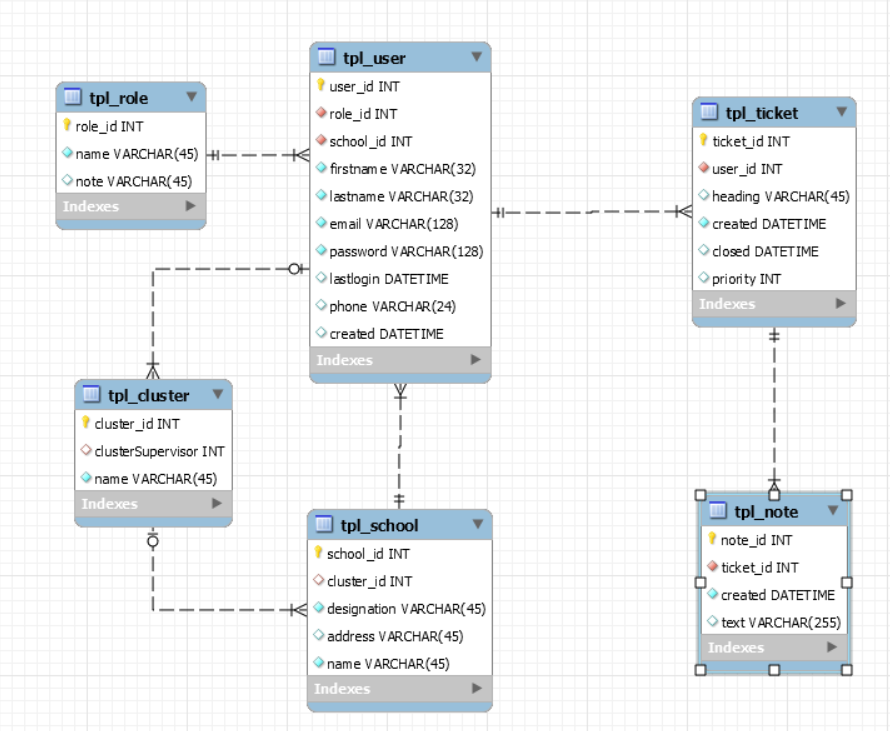
\includegraphics[scale=.8]{figures/EER-Diagramm-Java-EE-Anwendung.PNG}
	\caption{EER-Diagramm-Java-EE-Anwendung}
	\label{EER-Diagramm-Java-EE-Anwendung}
\end{figure}

\newpage

\subsubsection{tpl\_user}

In dieser Tabelle werden die User des Ticketsystems gehalten. Von einem User wird der Vorname, Nachname, E-Mail-Adresse und das Password gespeichert. Optional kann auch der letzte Login, die Telefonnummer und das Datum an dem er erstellt worden ist gespeichert werden.
Ein User muss einer Schule zugewiesen sein um vollständig im System registriert zu sein. Ein User kann auch ein Supervisor eines Clusters sein aber das ist optional.
WICHTIG: lastlogin und created werden nach folgender Form in der Datenbank gespeichert "YYYY-MM-DD HH:MM:SS".

\begin{table}[h]
	\begin{tabular}{|p{3.5cm}|p{4cm}|p{6.2cm}|}
		\hline
		\textbf{Column Name:} & \textbf{Datatype:} & \textbf{Content:}\\
		\hline
		user\_id & INT & Eindeutige ID des User. Dieser Wert ist rein technisch und hat  neben der Eindeutigkeit keine weitere Aussagekraft.\\
		\hline
		role\_id & INT( & Referenz zu der Rolle die der User besitzt\\
		\hline
		school\_id & INT &  Referenz zu der Schule vom User \\
		\hline
		firstname & VARCHAR(32) & Vorname des Users\\
		\hline
		lastname & VARCHAR(32) & Nachname des Users\\
		\hline
		email & VARCHAR(128) & E-Mail-Adresse des Users\\
		\hline
		password & VARCHAR(128) & Das Passwort des Users in Hash Form \\
		\hline
		lastlogin & DATETIME & Das Datum, in oben angegebener Form, an dem sich der User zuletzt angemeldet hat \\
		\hline
		password & VARCHAR(24) & Das Passwort des Users in Hash Form \\
		\hline
		created & DATETIME & Das Datum, in oben angegebener Form, an dem der User angelegt worden ist\\
		\hline
	\end{tabular}
	\caption{tab:tpl-user}
\end{table}
\label{tab:tpl_user}

\newpage

\subsubsection{tpl\_ticket}

In dieser Tabelle werden die erstellten Ticket des Ticketsystems gespeichert. Das Ticket wird genau einem User zugeordnet und kann mehrere Notizen(notes) haben. Des weiteren besteht ein Ticket aus einem Header, die Priorität und wann es erstellt und geschlossen worden ist.
WICHTIG: closed und created werden nach folgender Form in der Datenbank gespeichert "YYYY-MM-DD HH:MM:SS".

\begin{table}[h]
	\begin{tabular}{|p{3.5cm}|p{4cm}|p{6.2cm}|}
		\hline
		\textbf{Column Name:} & \textbf{Datatype:} & \textbf{Content:}\\
		\hline
		ticket\_id & INT & Eindeutige ID des Tickets. Dieser Wert ist rein technisch und hat neben der Eindeutigkeit keine weitere Aussagekraft.\\
		\hline
		user\_id & INT & Referenz zum User zu dem das Ticket gehört\\
		\hline
		heading & VARCHAR(45) &  Die Überschrift des Tickets\\
		\hline
		created & DATETIME & Das Datum, in oben angegebener Form, an dem das Ticket angelegt worden ist\\
		\hline
		closed & DATETIME & Das Datum, in oben angegebener Form, an dem das Ticket geschlossen worden ist\\
		\hline
		priority & INT & Hier wird die Priorität des Tickets angegeben. Kann eine Wert von 0-4 haben, der default Wert ist 0.\\
		\hline
	\end{tabular}
	\caption{tab:tpl-ticket}
\end{table}
\label{tab:tpl_ticket}

\newpage

\subsubsection{tpl\_note}

In dieser Tabelle werden die Notizen(notes) für die Tickets gespeichert. Jeder Notiz wird ein Ticket zugewiesen. Ein Ticket kann auch mehrere Notizen haben aber eine Notiz gehört immer genau zu einem Ticket. Eine Notiz besteht aus einem Text und einem Datum das angibt wann die Notiz erzeugt worden ist.
WICHTIG: created wird nach folgender Form in der Datenbank gespeichert "YYYY-MM-DD HH:MM:SS".

\begin{table}[h]
	\begin{tabular}{|p{3.5cm}|p{4cm}|p{6.2cm}|}
		\hline
		\textbf{Column Name:} & \textbf{Datatype:} & \textbf{Content:}\\
		\hline
		note\_id & INT & Eindeutige ID der Notiz. Dieser Wert ist rein technisch und hat neben der Eindeutigkeit keine weitere Aussagekraft.\\
		\hline
		ticket\_id & INT & Referenz zum Ticket dem diese Notiz angehört\\
		\hline
		created & DATETIME & Das Datum, in oben angegebener Form, an dem die Notiz angelegt worden ist\\
		\hline
		text & VARCHAR(255) & Ein Text der Informationen zum Ticket beinhaltet\\
		\hline
	\end{tabular}
	\caption{tab:tpl-note}
\end{table}
\label{tab:tpl_note}

\newpage

\subsubsection{tpl\_role}

In dieser Tabelle werden die Rollen gespeichert die ein User annehmen kann. Eine Rolle besteht lediglich aus einem Namen und einer Notiz. Ein User kann genau eine Rolle haben aber eine Rolle kann von mehreren User genutzt werden. 

\begin{table}[h]
	\begin{tabular}{|p{3.5cm}|p{4cm}|p{6.2cm}|}
		\hline
		\textbf{Column Name:} & \textbf{Datatype:} & \textbf{Content:}\\
		\hline
		role\_id & INT & Eindeutige ID der Rolle. Dieser Wert ist rein technisch und hat neben der Eindeutigkeit keine weitere Aussagekraft.\\
		\hline
		name & VARCHAR(45) & Name der Rolle\\
		\hline
		note & VARCHAR(45) & Informationen über die Rolle\\
		\hline
	\end{tabular}
	\caption{tab:tpl-role}
\end{table}
\label{tab:tpl_role}


\subsubsection{tpl\_school}

In dieser Tabelle werden die Schulen gespeichert die bei diesem Ticketsystem dabei sind.
Eine Schule wird mit Ihrer Bezeichnung, Adresse und Namen abgespeichert. Weiteres kann eine Schule einem Cluster zugeordnet werden. 

\begin{table}[h]
	\begin{tabular}{|p{3.5cm}|p{4cm}|p{6.2cm}|}
		\hline
		\textbf{Column Name:} & \textbf{Datatype:} & \textbf{Content:}\\
		\hline
		school\_id & INT & Eindeutige ID der Schule. Dieser Wert ist rein technisch und hat neben der Eindeutigkeit keine weitere Aussagekraft.\\
		\hline
		cluster\_id & INT & Referenz zu dem Cluster dem die Schule angehört\\
		\hline
		designation & VARCHAR(45) & Schulbezeichnung der Schule\\
		\hline
		address & VARCHAR(45) & Die Adresse der Schule\\
		\hline
		name & VARCHAR(45) & Name der Schule\\
		\hline
	\end{tabular}
	\caption{tab:tpl-school}
\end{table}
\label{tab:tpl_school}

\newpage

\subsubsection{tpl\_cluster}

In dieser Tabelle werden die Cluster festgelegt. Ein Cluster ist ein Mengen von Schule die zu einer Organisation zusammen geschlossen worden sind. Jeder Cluster hat einen Supervisor der für die Bearbeitung der anfallenden Ticket in diesem Cluster verantwortlich ist.
Der Supervisor wird per Referenz zur User-Tabelle festgelegt ein Cluster hat immer genau einen Supervisor. Zusätzlich wird noch ein Name für den Cluster festgelegt.

\begin{table}[h]
	\begin{tabular}{|p{3.5cm}|p{4cm}|p{6.2cm}|}
		\hline
		\textbf{Column Name:} & \textbf{Datatype:} & \textbf{Content:}\\
		\hline
		cluster\_id & INT & Eindeutige ID des Clusters. Dieser Wert ist rein technisch und hat neben der Eindeutigkeit keine weitere Aussagekraft.\\
		\hline
		clusterSupervisor & INT & Referenz zu dem User der in diesem Cluster der Supervisor ist\\
		\hline
		name & VARCHAR(45) & Name des Clusters\\
		\hline
	\end{tabular}
	\caption{tab:tpl-cluster}
\end{table}
\label{tab:tpl_cluster}

\newpage

\subsection{Beschreibung der Datenbankanbindung unserer Anwendung}

Die Datenbankanbindung wird durch die jdbc Api ermöglicht.

\begin{lstlisting}[language=JAVA, caption=Datenbankanbindung.java/getRoles-Methode, firstnumber=59]
public ArrayList getRoles()
{
ArrayList <tpl_role> roles = new ArrayList<>();

String value = "role_id";
String value1 = "name";
String value2 = "note";
try 
{
ResultSet rs = dbconnect().executeQuery("SELECT * FROM tpl_role");

while(rs.next())
{
tpl_role role = new tpl_role();

role.setName(rs.getString(value1));
role.setId(rs.getInt(value));
role.setNote(rs.getString(value2));

roles.add(role);
}
rs.close();
return roles;
} 
catch (SQLException ex) 
{
return null;
}
}

\end{lstlisting}

%todo: Datenbank Doku Gendern
%todo: Nummerierung der Tabellenname bei der Datenbank Doku
%todo: Formatieren der Tabellen
%todo: Einfügen der Datanbankanbindungs Doku OSTicket und Java ee Projekt
%todo: Einfügen der Datenbank Doku der Java ee Datenbank
%todo: Verschieben nach Kap. 2 (Vorstellung des Produktes; hier die JavaeEE Doku)
